\documentclass[../main.tex]{subfiles}

\begin{document}
\section{Projekt aplikacji}
W tej sekcji autor ma zamiar opisać architekturę aplikacji oraz przybliżyć w szczegółowy sposób oferowaną przez nią funkcjonalność.

\subsection{Architektura aplikacji}
Tworząc projekt korzystając z podejścia funkcyjnego wyodrębniamy jego część stanowiącą o logice biznesowej aplikacji. W tej części strukturyzujemy kod w taki sposób aby nie występowały w nim żadne efekty uboczne. Możemy powiedzieć, że stanowi to w całości funkcyjne "serce" / "szkielet" (ang. purely functional core) aplikacji\footnote{To jest z jakiegoś DevTalk'u który oglądałem, aczkolwiek muszę sobie jeszcze przypomnieć z jakiego :) }. Wykonywanie efektów ubocznych oddalamy tak daleko jak jest to tylko możliwe, aczkolwiek w pewnym momencie nie jesteśmy w stanie ich uniknąć. Na podstawie tego opisu kod projektu został podzielony w następujący sposób:\\
\begin{figure}[h]
    \centering
    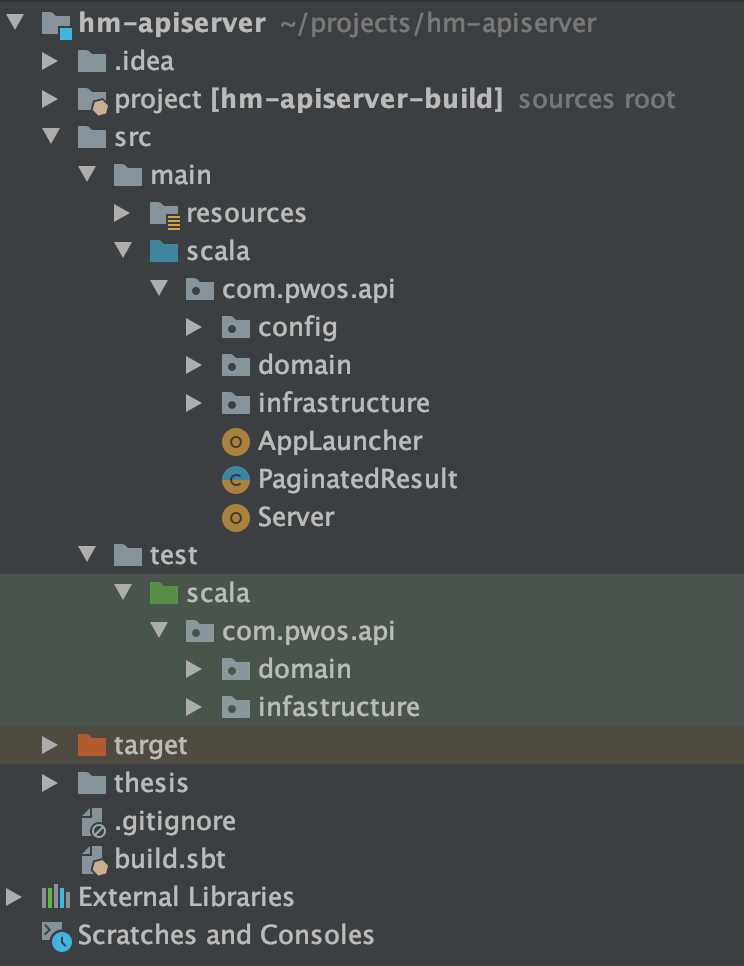
\includegraphics[width=0.4\textwidth]{images/01_project_structure.png}
    \caption{Struktura pakietów składających się na aplikację}
    \label{fig:struktura_pakietow}
\end{figure}\\
Kod aplikacji został podzielony na trzy główne pakiety:
\begin{itemize}
    \item config,
    \item domain,
    \item infrastructure.
\end{itemize}
\vspace{5ex}

Pakiet \textit{config} zawiera kod odpowiedzialny za wczytanie konfiguracji potrzebnej aplikacji do poprawnego działania. Składają się na nią zarówno ustawienia połączenia z bazą danych oraz interfejsu sieciowego aplikacji.\newline\newline
Całość kodu aplikacji znajdująca się w pakiecie \textit{domain} nie generuje żadnych efektów ubocznych. To właśnie w tym pakiecie zdefiniowana jest logika biznesowa w całości funkcyjny sposób.\newline\newline
Kod znajdujący się w pakiecie \textit{infrastructure} jest medium łączącym "czysty" (ang. pure) kod z sąsiedniego pakietu ze światem zewnętrznym. Ma to swoje odzwierciedlenie również w testach.\newline\newline


\subsubsection{Domain Driven Design}
Nie obędzie się też zapewne od wzmianki o DDD.

\subsubsection{Kontrollery (ang. controllers)}

\subsubsection{Services}
\subsubsection{DAOs}
\subsubsection{Models}

\vspace{15ex}






\subsection{Funkcjonalność aplikacji}

\subsubsection{Diagram ERD}

\subsubsection{Udostępnione endpointy}


\end{document}
